\chapter{Logikai függvények. Beágyazott függvények használata}
\thispagestyle{empty}


\section{Az IF függvény}

Az egyik leggyakrabban használt logikai függvény az IF. Egy
logikai vizsgálat eredményétől függően más-más
értéket ad eredményül. Három argumentuma van, az első
kötelező, a második és a harmadik elhagyható. Szintaxisa:\\ 
=IF(teszt; akkor érték; különben érték).

Az első paraméter logikai kifejezés,  tetszőleges
érték, illetve kifejezés, amely IGAZ vagy HAMIS értéket vehet
fel. Ebben az argumentumban a Calc bármelyik összehasonlító
operátorát használhatjuk. Ezeket \aref{ÖsszehasonlítóOp} táblázatban
láthatjuk.

\begin{table}[!h]
\begin{center}
\caption{Összehasonlító operátorok}\label{ÖsszehasonlítóOp}
\begin{tabular}{|c|l|}
\hline
\textbf{Operátor}&
\multicolumn{1}{c|}{\textbf{Név}} \\
\hline
=&
Egyenlő\\ \hline
\textgreater &
Nagyobb mint\\ \hline
\textless &
Kisebb mint\\ \hline
\textgreater= &
Nagyobb vagy egyenlő\\ \hline
\textless= &
Kisebb vagy egyenlő\\ \hline
\textless\textgreater &
Nem egyenlő\\ \hline
\end{tabular}
\end{center}
\end{table}

\Aref{ifFüggvény} ábrán látjuk, hogy az IF függvény az A1 cella
tartalmától függően a B1 cellában a
,,Felvételt nyert'' vagy az
,,elutasítva'' szöveget jeleníti
meg. Megvizsgálja, hogy a teszt eredménye igaz, vagy hamis. Igaz
esetén az a második paraméterben megadott szöveg jelenik meg,
hamis esetén a harmadikban.

\begin{figure}[!h]
\begin{center}
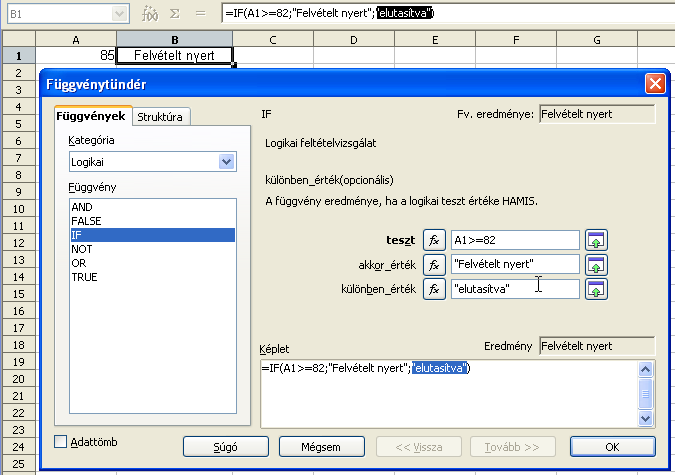
\includegraphics[width=13.199cm]{oocalcv1-img66.png}
\caption{IF függvény}\label{ifFüggvény}
\end{center}
\end{figure}

Az első paraméter kötelező, a függvénytündér az
ilyen paramétereket félkövér formázással jeleníti meg. A
második és a harmadik nem ilyen, ezeket opcionális vagy
elhagyható paramétereknek nevezzük. Esetünkben ha elhagynánk
a második és a harmadik paramétert, az IGAZ vagy a HAMIS
kifejezések valamelyike jelenne meg a B1 cellában.


\section{Egyéb logikai függvények}

Az \textbf{AND} logikai függvény akkor ad IGAZ eredményt, ha
minden argumentuma igaz. Például az =AND(A15;
A2>5) eredménye akkor IGAZ, ha mind az A1, mind az A2
tartalma nagyobb mint öt. Más esetben HAMIS.

Az \textbf{OR} logikai függvény IGAZ értéket ad vissza, ha
legalább egy argumentuma igaz. Például az =OR(A1>5;
A2>5) eredménye IGAZ, ha a két cella közül
legalább az egyik nagyobb mint öt. 

A \textbf{NOT} logikai függvény megfordítja a logikai értéket.


\section{12. feladat}

\begin{figure}[!h]
\begin{center}
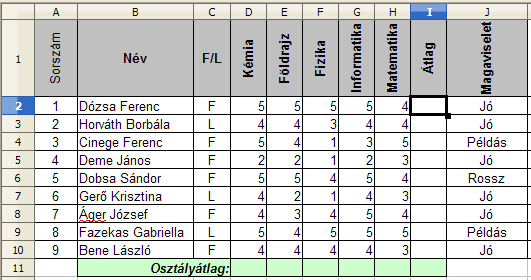
\includegraphics[width=11.048cm]{oocalcv1-img67.png}
\caption{12. feladat}\label{12-feladat}
\end{center}
\end{figure}

{\itshape
\Aref{12-feladat} ábrán egy osztály tanulóinak osztályzatait és
magaviseleti eredményeit látjuk. Készítsük el a képen
látható táblázatot a megfelelő formázásokkal.
Számítsuk ki minden tanuló átlagát az I~oszlopban és a
tantárgyak átlagát a 11. sorban. Az M oszlopban jelenjen meg a
,,Könyvjutalom'' szó azoknál a
tanulóknál, akik átlaga jobb mint 4,5 és magviselete Jó vagy
Példás.}

{\itshape
Mentsük a munkafüzetet calc03 néven, a munkalap neve legyen
Osztály.}

Az átlagértékek kiszámítása után a K2 cellában
válasszuk a függvénytündért. 

Esetünkben az IF, az AND és az OR függvényt is használni kell,
hogy a feladatot megoldjuk. Az IF függvény első argumentuma, le
kell hogy ellenőrizze, hogy a tanuló megfelel-e a
kritériumoknak. Ezek a kritériumok logikai függvényekkel
meghatározhatók. Tehát, az IF függvény első argumentuma
egy másik függvény lesz. A \textbf{teszt} szó utáni
$f_x$ feliratú gomb
ezt teszi lehetővé, ezzel a függvénybe további
függvényeket is beágyazhatunk.

{\itshape
Amikor egy függvény argumentumaként függvényt használunk,
azt beágyazott függvénynek nevezzük.}

\begin{figure}[!h]
\begin{center}
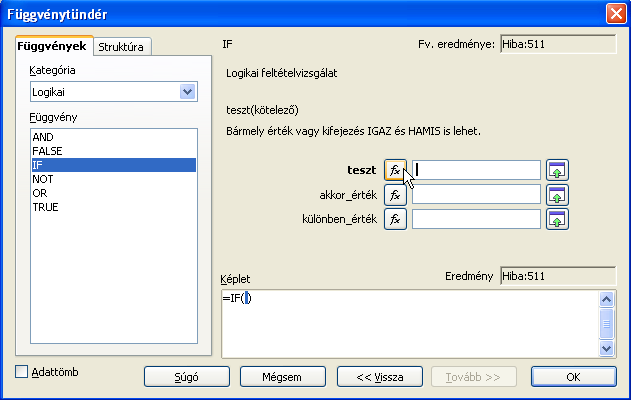
\includegraphics[width=13.999cm]{oocalcv1-img68.png}
\caption{12.  feladat --  IF függvény}\label{12-feladatIF}
\end{center}
\end{figure}

\begin{figure}[!h]
\begin{center}
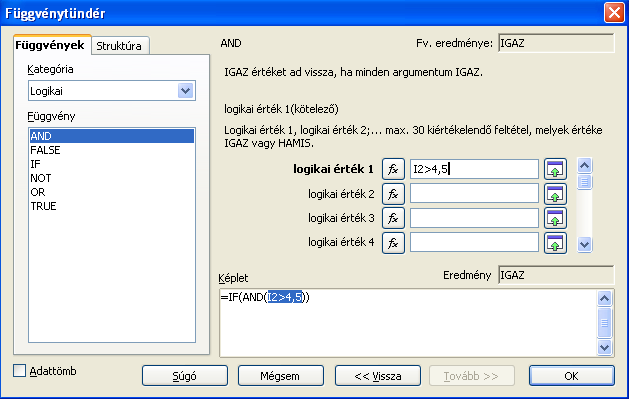
\includegraphics[width=13.999cm]{oocalcv1-img69.png}
\caption{12. feladat --  IF függvény argumentumok}\label{12-feladatArgum}
\end{center}
\end{figure}

Kattintsunk az $f_x$
feliratú gombra (\ref{12-feladatIF} ábra). A könyvjutalom elnyeréséhez
egyszerre két feltételnek kell megfelelnie a tanulónak, vagyis az
AND függvényt kell használnunk. Az egyik feltétel az, hogy a
tanuló átlaga jobb mint 4,5 (\ref{12-feladatArgum} ábra). A másik feltétel
viszont arról szól, hogy a két lehetőség közül
bármelyik esetén jár a könyvjutalom. Ismét beágyazott
függvényt kell használnunk.

Az AND függvény második paraméterének sorában válasszuk az
$f_x$ feliratú kapcsolót és az OR függvényt.

A függvények megkeresését megkönnyíti, hogy az első
kezdőbetűket leütve a Calc kiválasztja az adott
függvényt. Leginkább akkor hasznos, amikor egy
függvényről nem tudjuk, hogy melyik függvénykategóriában található.

Írjuk be az OR függvény argumentumait (\ref{12-feladatOR} ábra).

\begin{figure}[!h]
\begin{center}
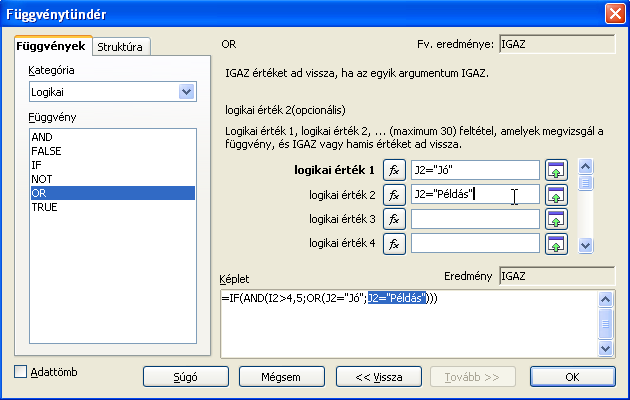
\includegraphics[width=13.999cm]{oocalcv1-img70.png}
\caption{12.  feladat --  OR függvény}\label{12-feladatOR}
\end{center}
\end{figure}

A függvénytündér Képlet ablakában látjuk az eddigi
lépések eredményeként létrehozott képletet. Ezek között
bármelyik függvényre kattintva újra módosíthatjuk azok
argumentumait. Válasszuk az IF függvényt és írjuk be a két
argumentumot (\ref{12-feladatIFArg} ábra).

\begin{figure}[!h]
\begin{center}
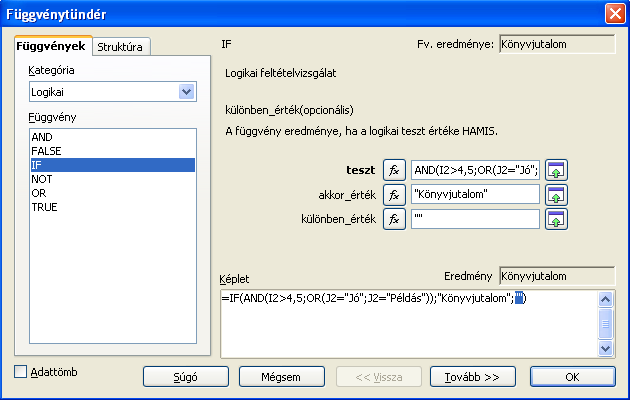
\includegraphics[width=13.999cm]{oocalcv1-img71.png}
\caption{12. feladat}\label{12-feladatIFArg}
\end{center}
\end{figure}

Az \textbf{akkor\_érték} ''Könyvjutalom'' lesz, a
\textbf{különben\_érték-}hez pedig írjunk két kettős
aposztrófot. Így a K oszlopban vagy a Könyvjutalom szó jelenik
meg, vagy üres marad a cella. Amennyiben nem írnánk semmit a
harmadik paraméterhez, a HAMIS szó jelenne meg az üres cella
helyett.

Másolással töltsük ki a K3:K10 tartományt.

A Calc igen áttekinthetően és látványosan jeleníti meg a
beágyazott függvényeket. Válasszuk ismét a K2 cellát és
kattintsunk a függvénytündér ikonjára. A
Függvénytündér a képlet struktúráját mutatja
(\ref{12-feladatFüggvénytündér} ábra).

\begin{figure}[!h]
\begin{center}
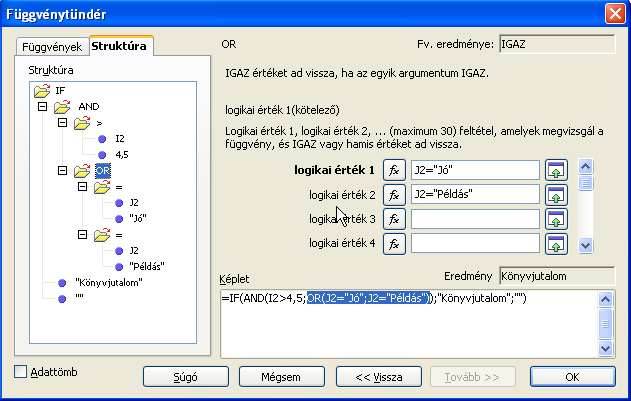
\includegraphics[width=13.999cm]{oocalcv1-img72.png}
\caption{12. feladat --  függvénytündér}\label{12-feladatFüggvénytündér}
\end{center}
\end{figure}

A Struktúra ablakban grafikusan látjuk a beágyazott
függvényeket és azok argumentumait.  Bármelyiket választva a
jobboldali ablakban látjuk az adott függvény részletes
beállításait és   eredményét is. \Aref{12-feladatFüggvénytündér} ábrán
látható, hogy az adott argumentumokkal az OR függvény
eredménye IGAZ, a teljes képlet pedig a
,,Könyvjutalom'' eredményt
adja.

\section[A SUMIF és a COUNTIF függvények]{A SUMIF és a
COUNTIF függvények}

Ezt a két függvényt nem a logikai, hanem a matematikai
függvények kategóriájában találjuk, de mivel mindkettő
feltételt tartalmaz, tekintsük át használatukat ebben a
fejezetben.

A SUMIF függvény segítségével összeadhatjuk a megadott
feltételnek megfelelő cellákat. Szintaxisa: SUMIF(tartomány;
feltételek; összegtartomány).

A harmadik paraméter elhagyható, ha a feltétel az
összegtartományra vonatkozik. Például a
=SUMIF(A1:A10;">5")
függvény az A1:A10 tartomány cellái közül azokat adja
össze, melyek nagyobbak ötnél.

\Aref{SUMIFFüggvény} ábrán látható példán azokat a cellákat adja össze
a SUMIF függvény az összegtartományból, amelyek fölött
esetünkben az ''alma'' szó
szerepel.

\begin{figure}[!h]
\begin{center}
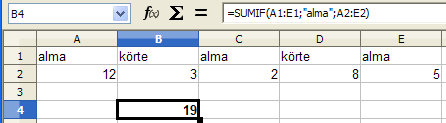
\includegraphics[width=10.799cm]{oocalcv1-img73.png}
\caption{SUMIF függvény}\label{SUMIFFüggvény}
\end{center}
\end{figure}

A COUNTIF függvénnyel összeszámolhatjuk egy tartomány bizonyos
feltételnek megfelelő elemeit.

Szintaxisa: COUNTIF(tartomány; feltételek). Mindkét paraméter
kötelező.

Például a =COUNTF(A1:A10;">5") megadja,
hogy hány olyan cella van az A1:A10 tartományban, amelyek ötnél
nagyobb számot tartalmaznak.


\section{13. feladat}
{\itshape
A 12. feladatot bővítsük két sorral. A 12. sorban
számítsuk ki a lányok átlagát, a 13-ban pedig a fiúk
átlagát minden tantárgyra.}

Ahhoz, hogy a D12 cellában kiszámítsuk a lányok átlagát
kémiából, össze kell adni a lányok jegyeit és elosztani a
lányok számával az osztályban.

A SUMIF függvénnyel összeadjuk azokat a számokat a D
oszlopból, amelyek mellett ''L''
betű van (\ref{13-feladatSUMIF} ábra).

\begin{figure}[!h]
\begin{center}
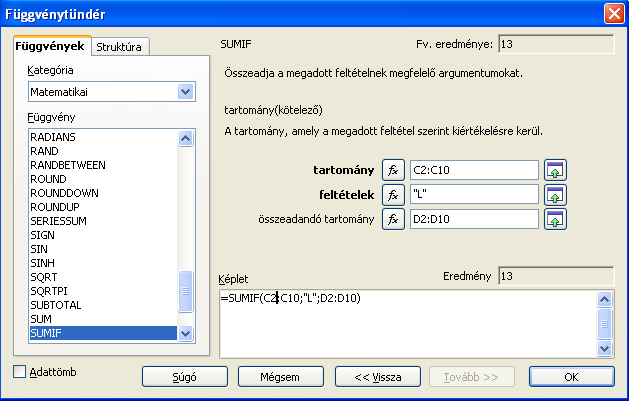
\includegraphics[width=13.999cm]{oocalcv1-img74.png}
\caption{13. feladat -- SUMIF függvény}\label{13-feladatSUMIF}
\end{center}
\end{figure}

A képlet után törtvonalat írva a COUNTIF függvénnyel
meghatározzuk az ''L'' betűk
darabszámát (\ref{13-feladatCOUNTIF} ábra).

\begin{figure}[!h]
\begin{center}
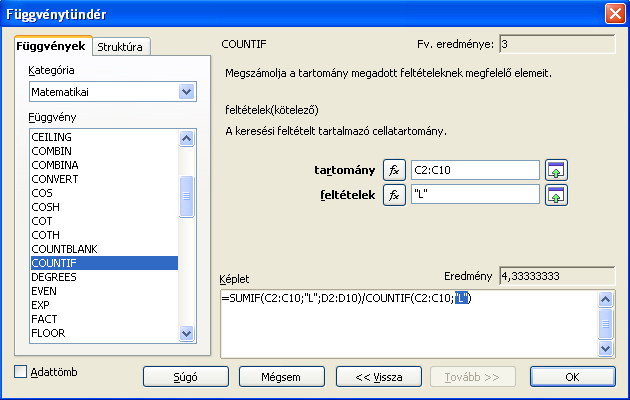
\includegraphics[width=13.999cm]{oocalcv1-img75.png}
\caption{13. feladat -- COUNTIF függvény}\label{13-feladatCOUNTIF}
\end{center}
\end{figure}

A képlet jobbra másolása előtt állítsuk be a megfelelő
vegyes cellahivatkozásokat. A végleges képlet
\aref{13-feladatMegoldás} ábrán látható.

\begin{figure}[!h]
\begin{center}
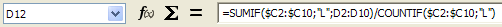
\includegraphics[width=12.28cm]{oocalcv1-img76.png}
\caption{13.  feladat -- megoldás}\label{13-feladatMegoldás}
\end{center}
\end{figure}

A fiúk átlagát megadó képlet csak annyiban tér el a
lányokétól, hogy a két
''L'' betűt
''F''-re kell cserélni. Ezért
egyszerűbb a D12-ben lévő képletet a beviteli sorban
kijelölni, másolni (Crtl+C), majd a D13 cellába beilleszteni
(Ctrl+V). Módosítva az említett argumentumot másoljuk jobbra a
képletet.

Az ebben a fejezetben tárgyalt függvényeket \aref{7-fejezetFüggvények}
táblázatban találjuk meg.


\begin{table}[!h]
\begin{center}
\caption{A fejezetben tárgyalt függvények}\label{7-fejezetFüggvények}
\begin{tabular}{|m{2.5cm}|m{8cm}|m{3cm}|}
\hline
 & & \multicolumn{1}{c|}{\textbf{Megfelelője a}} \\
\multicolumn{1}{|c|}{\textbf{A függvény}}&
\multicolumn{1}{c|}{\textbf{Funkciója}}&
\multicolumn{1}{c|}{\textbf{magyar}} \\
\multicolumn{1}{|c|}{\textbf{neve}} & &
\multicolumn{1}{c|}{\textbf{Microsoft}} \\
 & & \multicolumn{1}{c|}{\textbf{Excelben}} \\
\hline
IF & Logikai feltételvizsgálat. & HA\\ \hline
AND & Igaz értéket ad vissza, ha minden argumentuma igaz. & ÉS\\ \hline
OR & Igaz értéket ad vissza, ha egyik argumentuma igaz. & VAGY\\ \hline
NOT & Az argumentum értékét ellentettjére állítja. & NEM\\ \hline
SUMIF & Összeadja a megadott feltételnek megfelelő
argumentumokat. & SZUMHA\\ \hline
COUNTIF & Megszámolja a tartomány megadott feltételeknek
megfelelő elemeit. & DARABTELI\\ \hline
\end{tabular}
\end{center}
\end{table}

